% !TEX root = CartaPerali_Report.tex
\section{Models implementation}
\label{sec:models_implementation}

\noindent This section describes our models implementation. The code necessary to replicate our experiments is available at our GitHub repository. \red{ \it Possibly insert link here}
\subsection*{ \textbf {Data preprocessing and Features Extraction}} The first step to take in any KWS system is to extract features from our audio signal. For this task, the MFCC features were used. Thirteen-dimensional Mel-Frequency Cepstrum Coefficients (MFCC) frames are built using a 25ms window and a 10ms frame shift. \red{ \it Improve description here}

\subsection{ \textbf {CNN}} Our architecture is described in Fig. \ref{fig:CNN_schema}

\begin{figure}[h]
	\centering
	    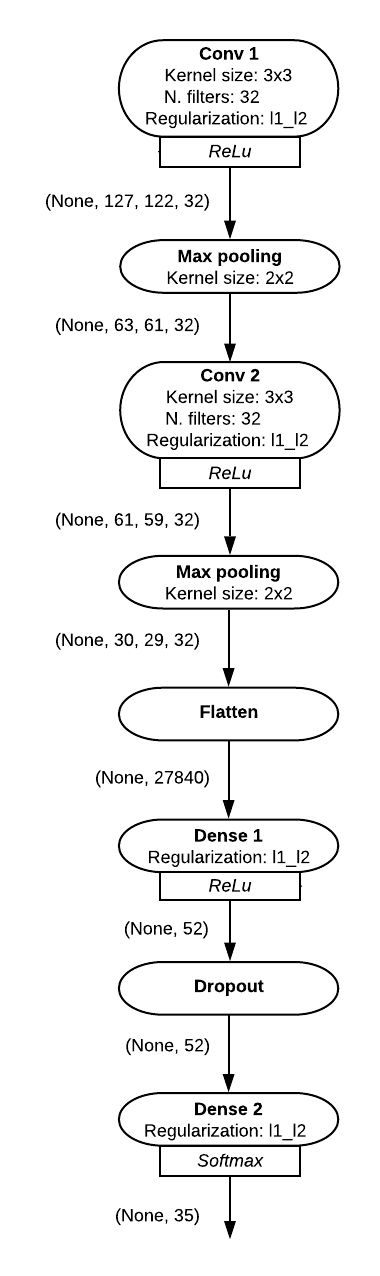
\includegraphics[width=0.25\textwidth]{CNN_schema}
	    \caption{CNN schema}
	    \label{fig:CNN_schema}
\end{figure}

\subsubsection{ \textbf {CNN subsection}} 
\subsubsection{ \textbf {CNN subsection}} 
\subsubsection{ \textbf {CNN subsection}} 

\subsection {\textbf {RNN}}
\subsubsection{ \textbf {RNN subsection}} 
\subsubsection{ \textbf {RNN subsection}} 
\subsubsection{ \textbf {RNN subsection}} 

\subsection {\textbf {HMM}}
\subsubsection{ \textbf {HMM subsection}} 
\subsubsection{ \textbf {HMM subsection}} 
\subsubsection{ \textbf {HMM subsection}} 


\red{
\begin{enumerate}
\item \textbf{On tailoring the paper structure to your needs:} The structure recommended for the previous sections is rather standard and could work for different papers with differing technical content, the structure and the paper content from here on highly depends on the type of paper, possibilities are: mostly based on theoretical analysis, showing experimental design/activity, proposing a new technique and analyzing its performance via experiments or simulation. For the HDA course we deal with machine learning and, in detail, with training and testing neural network architectures to perform some specific inference or classification task. The following structure and comments are specifically addressing this type of technical content.
\end{enumerate}}

\red{
\begin{remark}
\textbf{Why having this section:} With this section, we start the technical description with a {\it high level} introduction of your work (e.g., processing pipeline). Here, you do not have to necessarily go into the technical details of every block/algorithm of your design, this will be done later as the paper develops. What I would like to see here is a high level description of the approach, i.e., which processing blocks you used, what they do (in words) and how these were combined, etc. This section should introduce the reader to your design, explain the different parts/blocks, how they interact and why. You should not delve into technical details for each block, but you should rather explain the big picture. \MR{Besides a well written explanation, I often use a nice diagram containing the various blocks and detailing their interrelations.}
\end{remark} 
\noindent \textbf{Writing tips:} Sections, Figures and Tables are usually shortened as Sec., Fig., Tab. 
\begin{itemize}
\item \textbf{Cross referencing:} In Latex, cross referencing is easy. You need to label an object through the \texttt{\textbackslash label\{labelid\}} command and referencing it where you need it through the \texttt{\textbackslash ref\{labelid\}} command. 
\item \textbf{Suggestion:} I suggest to cross reference a table using \texttt{Tab.\mytexttilde\textbackslash ref\{tab:tableid\}}, the same holds for figures and sections, by just replacing ``\texttt{Tab.}'' with ``\texttt{Fig.}'' and ``\texttt{Sec.}''. Of course when defining the table, you need to add a Latex command \texttt{\textbackslash label\{tab:tableid\}} in the right place inside the table Latex environment to \mbox{cross-link} it. The tag \texttt{tab:tableid} is user defined and is the identifier that you associate with the table in question. You could call it \texttt{pippo} of you wish, but I recommend to use something like ``\texttt{tab:tableid}'' for tables, ``\texttt{eq:eqid}'' for equations, ``\texttt{sec:secid}'' for sections and so forth, where \texttt{tableid} has to be unique for each table in the document. The same applies to figures and all other objects. I guess you got the idea. This will lead to a neat Latex code and will facilitate cross referencing while avoiding duplicate labels, especially in large Latex documents (think of a book for example). 
\item \textbf{But what about the tilde?} This is a nice trick I have learned from a friend (many years ago from Prof. Frank Fitzek, now at TU Dresden). When you write \texttt{Tab.\mytexttilde\textbackslash ref\{tab:tableid\}} Latex knows that \texttt{Tab.} and the corresponding table number \texttt{\textbackslash ref\{tab:tableid\}} must be displayed within the same line, i.e., they can never be broken across lines. This is nice and desirable I believe. I always use it for all referenced material, including citations; example: ``As done in\texttt{\mytexttilde\textbackslash cite\{suppa-wu-2019\}}.''
\item \textbf{More about breaking stuff across lines} often times you have composed words, in line equations, etc. and for some reason you would like Latex to never break them across lines. Example: the Latex command \texttt{\textbackslash mbox\{Neural Networks (NN)\}} is processed by Latex so that ``\mbox{Neural Networks (NN)}'' is never broken across lines. I use this very often, also for inline equations that I do not want Latex to split across subsequent lines.
\end{itemize}
}


\section{Signals and Features}
\label{sec:model}

Being a machine learning paper, I would have here a section describing the signals you have been working on. If possible, you should describe, in order, 
\begin{enumerate}
\item the measurement setup (if relevant), how input data is formatted (e.g., vectors of fixed size measured at regular sampling times), 
\item how the signals were \mbox{pre-processed}, e.g., to remove noise, artifacts, fill gaps (missing points) or to re-interpolate the signals to represent them through a constant sampling rate, etc.
\item after this, you should describe how {\it feature vectors} were obtained from the \mbox{pre-processed} signals. If signals are {\it time series} this also implies stating the segmentation / windowing strategy that you adopted, to then describe how you obtained a feature vector for each time window. Also, if you use existing feature extraction approaches, you may want to briefly describe them as well, in addition to (and before) your own (possibly new) feature extraction method.
\end{enumerate}

\MR{Last but not least, this section should also contain information on how you have split the dataset into training, validation and test sets. This will be briefly recalled within the ``Results'' section.}

\section{Learning Framework}
\label{sec:learning_framework}

Here you finally describe the learning strategy / algorithm that you conceived and used to solve the problem at stake. A good diagram to exemplify how learning is carried out is often very useful. In this section, you should describe the learning model, its parameters, any optimization over a given parameter set, etc. You can organize this section into \mbox{sub-sections}. You are free to choose the most appropriate structure.

\begin{remark}
Note that the diagram that you put here differs from that of Section~\ref{sec:processing_architecture} as here you show the details of how your learning framework, or the core of it, is built. In Section~\ref{sec:processing_architecture} you instead provide a high-level description of the involved processing blocks, i.e., you describe the {\it processing flow} and the rationale behind it.
\end{remark}

\noindent \textbf{On math typesetting:} there are many Latex tricks that you should use to produce a high quality technical essay. A few are listed below, in random order:
\begin{itemize}
\item \textbf{Vectors and matrices:} $x$ is a scalar, whereas $\bm{x}$ (in bold) is a vector, and $\bm{X}$ is a matrix with elements $\bm{X} = [x_{ij}]$. For bold symbols you may use the \texttt{\textbackslash bm} Latex command, e.g., \texttt{\textbackslash bm(x)}.
\item \textbf{Operators:} such as $\max$, $\min$, $\arg\!\max$, $\arg\!\min$ and special functions such as $\log(\cdot)$, $\exp(\cdot)$, $\sin(\cdot)$, $\cos(\cdot)$ are obtained through specific latex commands \texttt{\textbackslash min}, \texttt{\textbackslash max}, \texttt{\textbackslash arg\textbackslash!min}, \texttt{\textbackslash arg\textbackslash!max}, \texttt{\textbackslash log}, \texttt{\textbackslash exp}, \texttt{\textbackslash sin}, \texttt{\textbackslash cos}, etc. Use them! $log$, $exp$, $min$, $sin$, $cos$, etc., look ugly.
\item \textbf{Sets} can be represented through calligraphic fonts, e.g., $\mathcal{S}$, $\mathcal{F}$, $\mathcal{B}$, etc., obtained using the Latex command \texttt{\textbackslash mathcal{\{S\}}}, etc.
\item \textbf{Equations:} for a single equation use the \texttt{equation} Latex environment. Example: 
\begin{equation}
\label{eq:sigmoid}
\sigma(x) = \frac{1}{1+e^{-x}}.
\end{equation} 
Now, using round brackets $($ and $)$ we get
\begin{equation}
\label{eq:sigmoid_comma}
\sigma(x) = (\frac{1}{1+e^{-x}}),
\end{equation} 
but this looks ugly, you should use ``\texttt{\textbackslash left (}'' for ``$($'' and ``\texttt{\textbackslash right )}'' for ``$)$'', obtaining
\begin{equation}
\sigma(x) = \left ( \frac{1}{1+e^{-x}} \right ).
\end{equation} 
\item \textbf{Punctuation:} Displayed equations are usually considered to be part of the text and, in turn, they will get the very same punctuation as if they were inline with the text (and part of the sentence). If the sentence ends with a displayed equation, the equation gets a period ``.'' right after it, see Eq.~(\ref{eq:sigmoid}). iI the equation is instead part of a running sentence, which is continued after it, then the equation may be ended by a ``,'' as in Eq.~(\ref{eq:sigmoid_comma}). Use the standard grammar rules and your good sense of flow to assess how equations should be punctuated, I usually read through as if they were plain text.
\end{itemize} 

